\documentclass[tikz,border=2pt]{standalone}
\usepackage{amsmath}
\usepackage{pgfplots}
\pgfplotsset{compat=1.18}

\begin{document}
% At a stationary point the sign of f'' decides: f''<0 (bending down) gives a local maximum,
% f''>0 (bending up) a local minimum; f''=0 decides nothing (x^3 at 0).
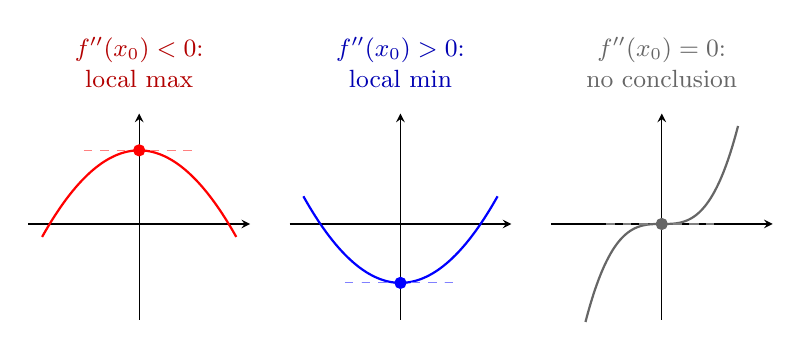
\begin{tikzpicture}
	\begin{axis}[
		name=a,
		axis lines=middle, xmin=-1.6, xmax=1.6, ymin=-1.3, ymax=1.5,
		xtick=\empty, ytick=\empty, samples=80, smooth, clip=false,
		width=4.4cm, height=4.2cm,
		title={$f''(x_0)<0$:\\ local max}, title style={font=\small, align=center, red!70!black}
		]
		\addplot[thick, red, domain=-1.4:1.4] {1-0.6*x^2};
		\addplot[only marks, mark=*, red] coordinates {(0,1)};
		\addplot[red!50, dashed, domain=-0.8:0.8] {1};
	\end{axis}
	\begin{axis}[
		name=b, at={(a.east)}, anchor=west, xshift=0.5cm,
		axis lines=middle, xmin=-1.6, xmax=1.6, ymin=-1.3, ymax=1.5,
		xtick=\empty, ytick=\empty, samples=80, smooth, clip=false,
		width=4.4cm, height=4.2cm,
		title={$f''(x_0)>0$:\\ local min}, title style={font=\small, align=center, blue!70!black}
		]
		\addplot[thick, blue, domain=-1.4:1.4] {-0.8+0.6*x^2};
		\addplot[only marks, mark=*, blue] coordinates {(0,-0.8)};
		\addplot[blue!50, dashed, domain=-0.8:0.8] {-0.8};
	\end{axis}
	\begin{axis}[
		at={(b.east)}, anchor=west, xshift=0.5cm,
		axis lines=middle, xmin=-1.6, xmax=1.6, ymin=-1.3, ymax=1.5,
		xtick=\empty, ytick=\empty, samples=80, smooth, clip=false,
		width=4.4cm, height=4.2cm,
		title={$f''(x_0)=0$:\\ no conclusion}, title style={font=\small, align=center, gray!80!black}
		]
		\addplot[thick, gray!80!black, domain=-1.1:1.1] {x^3};
		\addplot[only marks, mark=*, gray!80!black] coordinates {(0,0)};
		\addplot[gray, dashed, domain=-0.8:0.8] {0};
	\end{axis}
\end{tikzpicture}
\end{document}
